% documentation_FR.tex — WAC (Windows Artefacts Collector) user manual, French edition.
% The English edition is documentation_EN.tex, in this folder: both are maintained together,
% section for section.
%
% Build (XeLaTeX, two passes for the cover page and the table of contents):
%     latexmk -xelatex documentation_FR.tex
% The cover page is ../cover_FR.png.

\documentclass[11pt,a4paper,oneside]{report}

% ---------------------------------------------------------------- language and labels
\usepackage[french]{babel}
\newcommand{\wacdoctitle}{Documentation utilisateur}
\newcommand{\wacpageof}{sur}
\newcommand{\wacnotetitle}{À retenir}
\newcommand{\wacwarningtitle}{Attention}
% Layout shared with every WAC document.
% wac-style.tex — layout shared by every WAC document (user manuals, testing
% guides), French and English editions alike: one copy, so that they cannot
% drift apart.
%
% A document sets, BEFORE % wac-style.tex — layout shared by every WAC document (user manuals, testing
% guides), French and English editions alike: one copy, so that they cannot
% drift apart.
%
% A document sets, BEFORE % wac-style.tex — layout shared by every WAC document (user manuals, testing
% guides), French and English editions alike: one copy, so that they cannot
% drift apart.
%
% A document sets, BEFORE \input{../wac-style.tex}:
%   \usepackage[<language>]{babel}
%   \newcommand{\wacdoctitle}{...}      running header: "WAC — <title>"
%   \newcommand{\wacpageof}{...}        footer: "Page N <of> M"
%   \newcommand{\wacnotetitle}{...}     default title of the "note" box
%   \newcommand{\wacwarningtitle}{...}  default title of the "attention" box
% and AFTER it its \hypersetup (PDF title, author, subject).

% ---------------------------------------------------------------- fonts, language
\usepackage{fontspec}
\setmainfont{Noto Sans}
\setmonofont{DejaVu Sans Mono}[Scale=0.84]

% ---------------------------------------------------------------- layout
\usepackage[top=26mm,bottom=26mm,left=24mm,right=22mm,headheight=14pt]{geometry}
\usepackage{graphicx}
\graphicspath{{../}}
\usepackage{xcolor}
\usepackage{tikz}
\usepackage{booktabs,tabularx,longtable,array}
\usepackage{enumitem}
\usepackage{fancyhdr}
\usepackage{titlesec}
\usepackage[most]{tcolorbox}
\usepackage{listings}
\usepackage{url}
\usepackage{lastpage}
\usepackage[hidelinks,unicode,pdfpagelabels]{hyperref}

% Colours sampled from the cover page
\definecolor{marine}{HTML}{0A1A33}
\definecolor{bleu}{HTML}{2F6DB5}
\definecolor{accent}{HTML}{1F66D1}
\definecolor{fond}{HTML}{EEF3FA}
\definecolor{alerte}{HTML}{B3261E}
\definecolor{fondalerte}{HTML}{FBEDEC}
\definecolor{gris}{HTML}{5B6573}

\setlength{\parindent}{0pt}
\setlength{\parskip}{0.55em}
\linespread{1.08}
\setlist{itemsep=0.25em,topsep=0.35em}
\urlstyle{tt}
\renewcommand{\arraystretch}{1.25}
% Left-aligned table columns: justified narrow columns opened wide gaps
% between words.
\newcolumntype{L}[1]{>{\raggedright\arraybackslash}p{#1}}
% Monospaced file and field names cannot be hyphenated: let the line's spaces
% stretch instead.
\setlength{\emergencystretch}{3em}

% Headings
\titleformat{\chapter}[display]
  {\color{marine}\bfseries\raggedright}
  {\color{bleu}\large\MakeUppercase{\chaptertitlename}~\thechapter}
  {0.3em}
  {\Huge}[{\color{accent}\titlerule[2pt]}]
\titlespacing*{\chapter}{0pt}{0pt}{1.6em}
\titleformat{\section}{\color{marine}\Large\bfseries}{\color{bleu}\thesection}{0.8em}{}
\titleformat{\subsection}{\color{marine}\large\bfseries}{\color{bleu}\thesubsection}{0.7em}{}
\titleformat{\subsubsection}{\color{bleu}\normalsize\bfseries}{}{0em}{}

% Headers and footers
\pagestyle{fancy}
\fancyhf{}
\fancyhead[L]{\small\color{gris}WAC — \wacdoctitle}
\fancyhead[R]{\small\color{gris}\leftmark}
% Footer: "Page N of M" (the word set by \wacpageof), readable. A bare, small, light-grey number went
% unnoticed.
\newcommand{\piedpage}{\small\color{marine}\textbf{Page \thepage}\ \wacpageof\ \pageref*{LastPage}}
\fancyfoot[C]{\piedpage}
\renewcommand{\footrulewidth}{0.4pt}
\renewcommand{\footrule}{\hbox to\headwidth{\color{fond}\leaders\hrule height \footrulewidth\hfill}}
\renewcommand{\headrulewidth}{0.4pt}
\renewcommand{\headrule}{\hbox to\headwidth{\color{fond}\leaders\hrule height \headrulewidth\hfill}}
\renewcommand{\chaptermark}[1]{\markboth{#1}{}}
\fancypagestyle{plain}{\fancyhf{}\fancyfoot[C]{\piedpage}\renewcommand{\headrulewidth}{0pt}}

% Boxes
\newtcolorbox{note}[1][\wacnotetitle]{enhanced,breakable,colback=fond,colframe=bleu,
  boxrule=0pt,leftrule=3pt,arc=0pt,left=8pt,right=8pt,top=6pt,bottom=6pt,
  title={\bfseries #1},coltitle=bleu,colbacktitle=fond,attach title to upper={\par\smallskip}}
\newtcolorbox{attention}[1][\wacwarningtitle]{enhanced,breakable,colback=fondalerte,colframe=alerte,
  boxrule=0pt,leftrule=3pt,arc=0pt,left=8pt,right=8pt,top=6pt,bottom=6pt,
  title={\bfseries #1},coltitle=alerte,colbacktitle=fondalerte,attach title to upper={\par\smallskip}}

% Code
\lstset{basicstyle=\ttfamily\small,columns=fullflexible,keepspaces=true,
  backgroundcolor=\color{fond},frame=l,framerule=3pt,rulecolor=\color{bleu},
  xleftmargin=9pt,framexleftmargin=6pt,aboveskip=0.8em,belowskip=0.8em,
  breaklines=true,breakatwhitespace=false,showstringspaces=false,
  literate={é}{{\'e}}1 {è}{{\`e}}1 {à}{{\`a}}1 {ê}{{\^e}}1 {ô}{{\^o}}1 {ç}{{\c c}}1
           {É}{{\'E}}1 {—}{{---}}1 {’}{{'}}1 {…}{{...}}1 {«}{{\guillemotleft}}1 {»}{{\guillemotright}}1}

% Shortcuts
\newcommand{\wac}{\textsc{wac}}
\newcommand{\opt}[1]{\texttt{-{}-#1}}
\newcommand{\champ}[1]{\texttt{#1}}
\newcommand{\fichier}[1]{\texttt{#1}}
:
%   \usepackage[<language>]{babel}
%   \newcommand{\wacdoctitle}{...}      running header: "WAC — <title>"
%   \newcommand{\wacpageof}{...}        footer: "Page N <of> M"
%   \newcommand{\wacnotetitle}{...}     default title of the "note" box
%   \newcommand{\wacwarningtitle}{...}  default title of the "attention" box
% and AFTER it its \hypersetup (PDF title, author, subject).

% ---------------------------------------------------------------- fonts, language
\usepackage{fontspec}
\setmainfont{Noto Sans}
\setmonofont{DejaVu Sans Mono}[Scale=0.84]

% ---------------------------------------------------------------- layout
\usepackage[top=26mm,bottom=26mm,left=24mm,right=22mm,headheight=14pt]{geometry}
\usepackage{graphicx}
\graphicspath{{../}}
\usepackage{xcolor}
\usepackage{tikz}
\usepackage{booktabs,tabularx,longtable,array}
\usepackage{enumitem}
\usepackage{fancyhdr}
\usepackage{titlesec}
\usepackage[most]{tcolorbox}
\usepackage{listings}
\usepackage{url}
\usepackage{lastpage}
\usepackage[hidelinks,unicode,pdfpagelabels]{hyperref}

% Colours sampled from the cover page
\definecolor{marine}{HTML}{0A1A33}
\definecolor{bleu}{HTML}{2F6DB5}
\definecolor{accent}{HTML}{1F66D1}
\definecolor{fond}{HTML}{EEF3FA}
\definecolor{alerte}{HTML}{B3261E}
\definecolor{fondalerte}{HTML}{FBEDEC}
\definecolor{gris}{HTML}{5B6573}

\setlength{\parindent}{0pt}
\setlength{\parskip}{0.55em}
\linespread{1.08}
\setlist{itemsep=0.25em,topsep=0.35em}
\urlstyle{tt}
\renewcommand{\arraystretch}{1.25}
% Left-aligned table columns: justified narrow columns opened wide gaps
% between words.
\newcolumntype{L}[1]{>{\raggedright\arraybackslash}p{#1}}
% Monospaced file and field names cannot be hyphenated: let the line's spaces
% stretch instead.
\setlength{\emergencystretch}{3em}

% Headings
\titleformat{\chapter}[display]
  {\color{marine}\bfseries\raggedright}
  {\color{bleu}\large\MakeUppercase{\chaptertitlename}~\thechapter}
  {0.3em}
  {\Huge}[{\color{accent}\titlerule[2pt]}]
\titlespacing*{\chapter}{0pt}{0pt}{1.6em}
\titleformat{\section}{\color{marine}\Large\bfseries}{\color{bleu}\thesection}{0.8em}{}
\titleformat{\subsection}{\color{marine}\large\bfseries}{\color{bleu}\thesubsection}{0.7em}{}
\titleformat{\subsubsection}{\color{bleu}\normalsize\bfseries}{}{0em}{}

% Headers and footers
\pagestyle{fancy}
\fancyhf{}
\fancyhead[L]{\small\color{gris}WAC — \wacdoctitle}
\fancyhead[R]{\small\color{gris}\leftmark}
% Footer: "Page N of M" (the word set by \wacpageof), readable. A bare, small, light-grey number went
% unnoticed.
\newcommand{\piedpage}{\small\color{marine}\textbf{Page \thepage}\ \wacpageof\ \pageref*{LastPage}}
\fancyfoot[C]{\piedpage}
\renewcommand{\footrulewidth}{0.4pt}
\renewcommand{\footrule}{\hbox to\headwidth{\color{fond}\leaders\hrule height \footrulewidth\hfill}}
\renewcommand{\headrulewidth}{0.4pt}
\renewcommand{\headrule}{\hbox to\headwidth{\color{fond}\leaders\hrule height \headrulewidth\hfill}}
\renewcommand{\chaptermark}[1]{\markboth{#1}{}}
\fancypagestyle{plain}{\fancyhf{}\fancyfoot[C]{\piedpage}\renewcommand{\headrulewidth}{0pt}}

% Boxes
\newtcolorbox{note}[1][\wacnotetitle]{enhanced,breakable,colback=fond,colframe=bleu,
  boxrule=0pt,leftrule=3pt,arc=0pt,left=8pt,right=8pt,top=6pt,bottom=6pt,
  title={\bfseries #1},coltitle=bleu,colbacktitle=fond,attach title to upper={\par\smallskip}}
\newtcolorbox{attention}[1][\wacwarningtitle]{enhanced,breakable,colback=fondalerte,colframe=alerte,
  boxrule=0pt,leftrule=3pt,arc=0pt,left=8pt,right=8pt,top=6pt,bottom=6pt,
  title={\bfseries #1},coltitle=alerte,colbacktitle=fondalerte,attach title to upper={\par\smallskip}}

% Code
\lstset{basicstyle=\ttfamily\small,columns=fullflexible,keepspaces=true,
  backgroundcolor=\color{fond},frame=l,framerule=3pt,rulecolor=\color{bleu},
  xleftmargin=9pt,framexleftmargin=6pt,aboveskip=0.8em,belowskip=0.8em,
  breaklines=true,breakatwhitespace=false,showstringspaces=false,
  literate={é}{{\'e}}1 {è}{{\`e}}1 {à}{{\`a}}1 {ê}{{\^e}}1 {ô}{{\^o}}1 {ç}{{\c c}}1
           {É}{{\'E}}1 {—}{{---}}1 {’}{{'}}1 {…}{{...}}1 {«}{{\guillemotleft}}1 {»}{{\guillemotright}}1}

% Shortcuts
\newcommand{\wac}{\textsc{wac}}
\newcommand{\opt}[1]{\texttt{-{}-#1}}
\newcommand{\champ}[1]{\texttt{#1}}
\newcommand{\fichier}[1]{\texttt{#1}}
:
%   \usepackage[<language>]{babel}
%   \newcommand{\wacdoctitle}{...}      running header: "WAC — <title>"
%   \newcommand{\wacpageof}{...}        footer: "Page N <of> M"
%   \newcommand{\wacnotetitle}{...}     default title of the "note" box
%   \newcommand{\wacwarningtitle}{...}  default title of the "attention" box
% and AFTER it its \hypersetup (PDF title, author, subject).

% ---------------------------------------------------------------- fonts, language
\usepackage{fontspec}
\setmainfont{Noto Sans}
\setmonofont{DejaVu Sans Mono}[Scale=0.84]

% ---------------------------------------------------------------- layout
\usepackage[top=26mm,bottom=26mm,left=24mm,right=22mm,headheight=14pt]{geometry}
\usepackage{graphicx}
\graphicspath{{../}}
\usepackage{xcolor}
\usepackage{tikz}
\usepackage{booktabs,tabularx,longtable,array}
\usepackage{enumitem}
\usepackage{fancyhdr}
\usepackage{titlesec}
\usepackage[most]{tcolorbox}
\usepackage{listings}
\usepackage{url}
\usepackage{lastpage}
\usepackage[hidelinks,unicode,pdfpagelabels]{hyperref}

% Colours sampled from the cover page
\definecolor{marine}{HTML}{0A1A33}
\definecolor{bleu}{HTML}{2F6DB5}
\definecolor{accent}{HTML}{1F66D1}
\definecolor{fond}{HTML}{EEF3FA}
\definecolor{alerte}{HTML}{B3261E}
\definecolor{fondalerte}{HTML}{FBEDEC}
\definecolor{gris}{HTML}{5B6573}

\setlength{\parindent}{0pt}
\setlength{\parskip}{0.55em}
\linespread{1.08}
\setlist{itemsep=0.25em,topsep=0.35em}
\urlstyle{tt}
\renewcommand{\arraystretch}{1.25}
% Left-aligned table columns: justified narrow columns opened wide gaps
% between words.
\newcolumntype{L}[1]{>{\raggedright\arraybackslash}p{#1}}
% Monospaced file and field names cannot be hyphenated: let the line's spaces
% stretch instead.
\setlength{\emergencystretch}{3em}

% Headings
\titleformat{\chapter}[display]
  {\color{marine}\bfseries\raggedright}
  {\color{bleu}\large\MakeUppercase{\chaptertitlename}~\thechapter}
  {0.3em}
  {\Huge}[{\color{accent}\titlerule[2pt]}]
\titlespacing*{\chapter}{0pt}{0pt}{1.6em}
\titleformat{\section}{\color{marine}\Large\bfseries}{\color{bleu}\thesection}{0.8em}{}
\titleformat{\subsection}{\color{marine}\large\bfseries}{\color{bleu}\thesubsection}{0.7em}{}
\titleformat{\subsubsection}{\color{bleu}\normalsize\bfseries}{}{0em}{}

% Headers and footers
\pagestyle{fancy}
\fancyhf{}
\fancyhead[L]{\small\color{gris}WAC — \wacdoctitle}
\fancyhead[R]{\small\color{gris}\leftmark}
% Footer: "Page N of M" (the word set by \wacpageof), readable. A bare, small, light-grey number went
% unnoticed.
\newcommand{\piedpage}{\small\color{marine}\textbf{Page \thepage}\ \wacpageof\ \pageref*{LastPage}}
\fancyfoot[C]{\piedpage}
\renewcommand{\footrulewidth}{0.4pt}
\renewcommand{\footrule}{\hbox to\headwidth{\color{fond}\leaders\hrule height \footrulewidth\hfill}}
\renewcommand{\headrulewidth}{0.4pt}
\renewcommand{\headrule}{\hbox to\headwidth{\color{fond}\leaders\hrule height \headrulewidth\hfill}}
\renewcommand{\chaptermark}[1]{\markboth{#1}{}}
\fancypagestyle{plain}{\fancyhf{}\fancyfoot[C]{\piedpage}\renewcommand{\headrulewidth}{0pt}}

% Boxes
\newtcolorbox{note}[1][\wacnotetitle]{enhanced,breakable,colback=fond,colframe=bleu,
  boxrule=0pt,leftrule=3pt,arc=0pt,left=8pt,right=8pt,top=6pt,bottom=6pt,
  title={\bfseries #1},coltitle=bleu,colbacktitle=fond,attach title to upper={\par\smallskip}}
\newtcolorbox{attention}[1][\wacwarningtitle]{enhanced,breakable,colback=fondalerte,colframe=alerte,
  boxrule=0pt,leftrule=3pt,arc=0pt,left=8pt,right=8pt,top=6pt,bottom=6pt,
  title={\bfseries #1},coltitle=alerte,colbacktitle=fondalerte,attach title to upper={\par\smallskip}}

% Code
\lstset{basicstyle=\ttfamily\small,columns=fullflexible,keepspaces=true,
  backgroundcolor=\color{fond},frame=l,framerule=3pt,rulecolor=\color{bleu},
  xleftmargin=9pt,framexleftmargin=6pt,aboveskip=0.8em,belowskip=0.8em,
  breaklines=true,breakatwhitespace=false,showstringspaces=false,
  literate={é}{{\'e}}1 {è}{{\`e}}1 {à}{{\`a}}1 {ê}{{\^e}}1 {ô}{{\^o}}1 {ç}{{\c c}}1
           {É}{{\'E}}1 {—}{{---}}1 {’}{{'}}1 {…}{{...}}1 {«}{{\guillemotleft}}1 {»}{{\guillemotright}}1}

% Shortcuts
\newcommand{\wac}{\textsc{wac}}
\newcommand{\opt}[1]{\texttt{-{}-#1}}
\newcommand{\champ}[1]{\texttt{#1}}
\newcommand{\fichier}[1]{\texttt{#1}}


\hypersetup{pdftitle={WAC — Documentation utilisateur},
  pdfauthor={Centre d'Excellence Cyberdéfense Aérospatiale (CEC)},
  pdfsubject={Logiciel de prélèvement d'artefacts Windows pour l'investigation numérique}}

\begin{document}

% ============================================================ COVER PAGE
\pagenumbering{roman}
\begin{titlepage}
\thispagestyle{empty}
\begin{tikzpicture}[remember picture,overlay]
  \node[inner sep=0pt] at (current page.center)
    {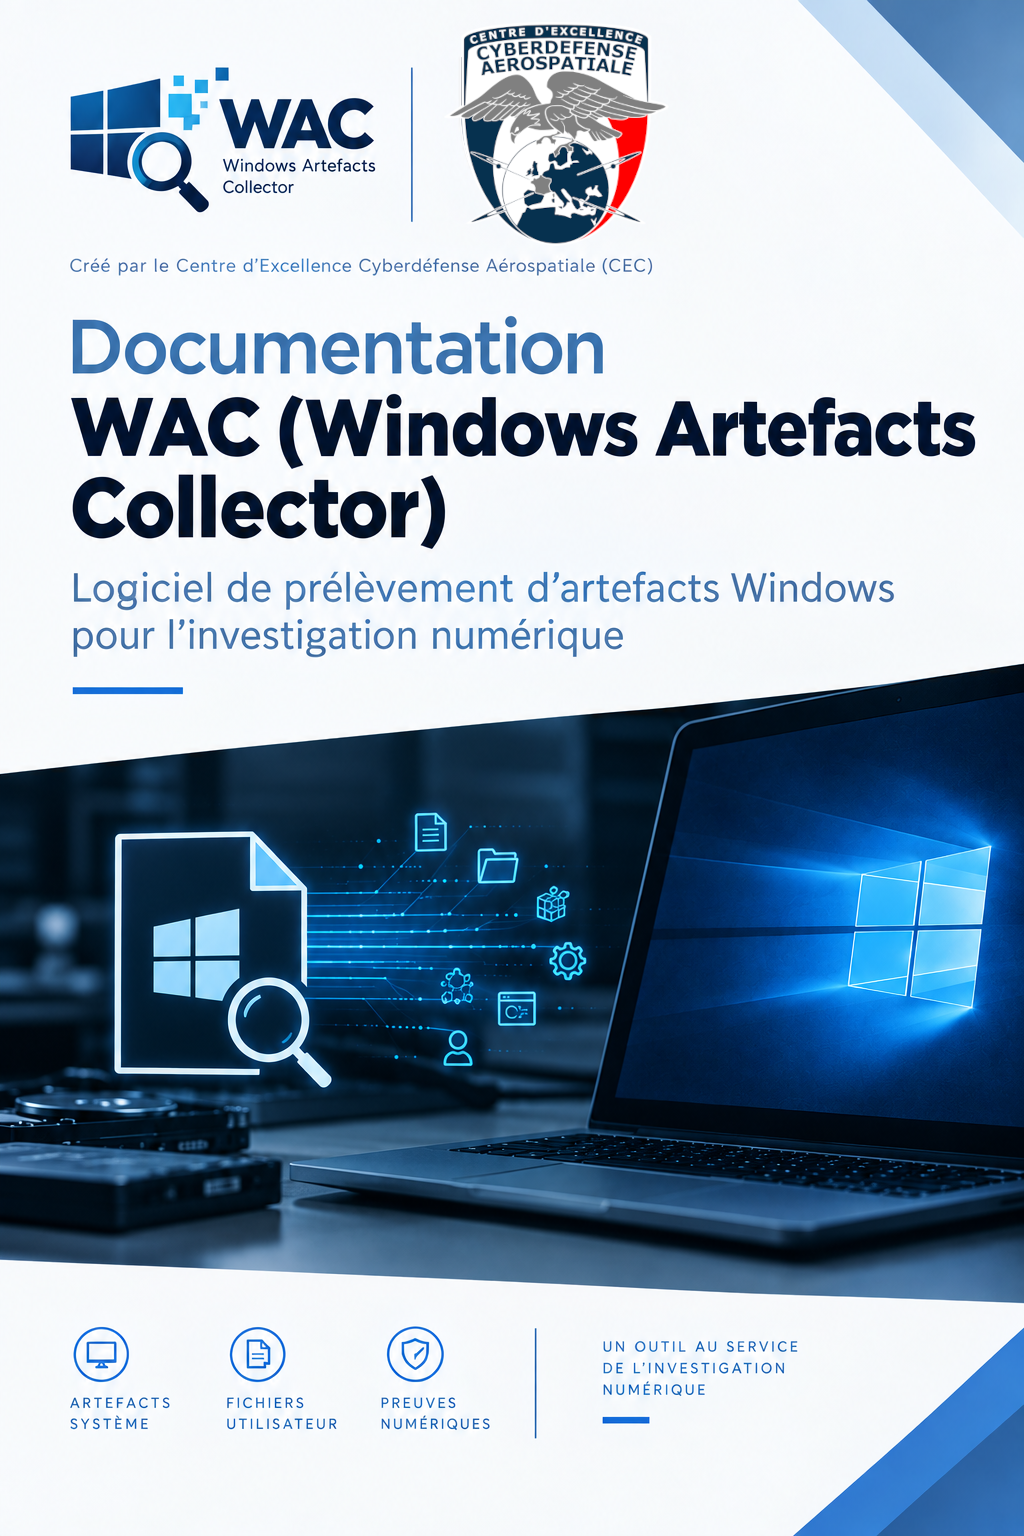
\includegraphics[width=\paperwidth]{cover_FR.png}};
\end{tikzpicture}
\end{titlepage}

% ============================================================ INFORMATION PAGE
\thispagestyle{empty}
\vspace*{\fill}
{\color{marine}\Large\bfseries WAC — Windows Artefacts Collector}\par
{\color{bleu}Documentation utilisateur}\par
\medskip
\begin{tabular}{@{}ll@{}}
Version du logiciel & 1.3.1 \\
Édition du document & septembre 2026 \\
Éditeur & Centre d'Excellence Cyberdéfense Aérospatiale (CEC) \\
        & École de l'air et de l'espace, base aérienne 701, Salon-de-Provence \\
\end{tabular}

\bigskip
{\small\color{gris}Ce document décrit l'emploi de \wac{} : préparation, exécution
d'une collecte, lecture et vérification des résultats, et traces laissées sur la
machine examinée. Les mesures citées ont été relevées sur une machine virtuelle
Windows~11 de test ; elles donnent des ordres de grandeur, pas des
engagements.}
\vspace*{2cm}
\clearpage

% Numbering starts at 1 with the table of contents; only the cover page and the
% information page, which have no footer, are left out of it.
\pagenumbering{arabic}
\tableofcontents

% ============================================================ 1
\chapter{Présentation}

\section{À quoi sert WAC}

\wac{} prélève, sur un poste Windows en fonctionnement, les artefacts utiles à
une investigation numérique : base de registre, journaux d'événements, fichiers
Prefetch, raccourcis et listes de sauts, tâches planifiées, services, comptes,
processus et sessions. Il les restitue sous forme de fichiers \textbf{JSON},
prêts à être analysés ou versés dans une chaîne de traitement.

Il s'exécute depuis une clé USB, sans installation, et écrit tout ce qu'il
produit sur cette clé.

\section{Le principe directeur : une empreinte minimale}

Examiner une machine la modifie. Chaque outil lancé laisse des traces : fichiers
ouverts dont la date de dernier accès change, services sollicités qui écrivent
dans les journaux, clés de registre lues par l'API. Ces traces se mêlent à celles
que l'on cherche.

\wac{} est conçu pour que ce qu'il laisse derrière lui soit aussi proche de rien
que la tâche le permet, et pour que \textbf{ce qu'il ne peut pas éviter soit
écrit}. Concrètement :

\begin{itemize}
  \item le disque est lu \textbf{directement}, en lecture seule, sans ouvrir aucun
        fichier par le système : aucune date d'accès n'est modifiée ;
  \item aucune clé du registre de la machine n'est ouverte : les ruches sont
        copiées, puis lues sur la copie ;
  \item aucun cliché instantané (VSS), aucun appel COM ou WMI, aucun service de
        journalisation n'est sollicité ;
  \item rien n'est écrit sur le disque examiné ;
  \item chaque opération est consignée, avec la trace qu'elle est censée laisser,
        dans \fichier{investigation.json}.
\end{itemize}

\section{Ce que WAC ne fait pas}

\begin{itemize}
  \item \wac{} \textbf{n'analyse pas} : il prélève et met en forme. L'interprétation
        revient à l'analyste.
  \item Il ne réalise pas d'image complète du disque : il extrait les fichiers
        porteurs d'artefacts.
  \item Il ne capture pas la mémoire vive. Les seules données volatiles relevées
        sont la liste des processus, les sessions ouvertes et l'état des
        services.
\end{itemize}

% ============================================================ 2
\chapter{Principes de fonctionnement}

\section{Lecture directe du disque}

\wac{} ouvre le volume (\path|\\.\C:|) en lecture seule, parcourt lui-même la
table des fichiers NTFS (\path|$MFT|) et en extrait le contenu des fichiers
utiles. Le système ne voit aucune ouverture de fichier : ni date d'accès mise à
jour, ni parcours de répertoire, ni verrou.

Cette lecture prend en charge les particularités de NTFS que Windows masque
d'ordinaire :

\begin{description}[style=nextline,leftmargin=1.2em]
  \item[Compression NTFS] Windows~11 compresse notamment le dossier des journaux
        d'événements. \wac{} les décompresse lui-même.
  \item[Compact OS (WOF)] Les binaires système de Windows~10 et~11 sont stockés
        compressés dans un flux caché ; vus par l'API, ils paraissent ordinaires.
        \wac{} les décompresse (variantes XPRESS).
  \item[Attributs éclatés] Un fichier très fragmenté voit ses informations
        réparties sur plusieurs enregistrements ; \wac{} les réunit.
  \item[Fichiers préalloués] Au-delà de la longueur de données valides, NTFS
        rend des zéros, même si le disque contient encore les restes d'anciens
        fichiers. \wac{} fait de même : le contenu extrait est celui que verrait
        toute acquisition ordinaire, et son empreinte aussi.
\end{description}

\section{Consigne et travail}

Une pièce à conviction numérique ne s'examine jamais sur elle-même : on en fait
une copie, on la scelle, et l'on travaille sur une seconde copie. Si l'analyse
abîme quelque chose, la copie scellée demeure et l'opération peut être refaite.

\wac{} applique cette procédure à \textbf{tous} les fichiers extraits, y compris
ceux qu'il ne modifie pas :

\begin{description}[style=nextline,leftmargin=1.2em]
  \item[\fichier{exhibits/}] les copies brutes, telles que lues sur le volume. Ce
        répertoire n'est plus jamais rouvert en écriture après l'extraction. Il
        contient le manifeste qui identifie chaque pièce, et le sceau du
        manifeste.
  \item[\fichier{working/}] les copies de travail, recopiées depuis la consigne
        et vérifiées par empreinte. C'est ici que sont faites les seules
        modifications (rejeu des journaux de transaction des ruches), et c'est ici
        que lisent tous les collecteurs.
\end{description}

\begin{note}
Chaque fichier extrait est donc écrit \textbf{deux fois} sur le support de
collecte. Prévoyez la place correspondante (voir
section~\ref{sec:place}).
\end{note}

\section{Ruches du registre et journaux de transaction}

Une ruche copiée sur une machine en fonctionnement ne contient pas les dernières
modifications : elles sont encore dans ses journaux de transaction
(\fichier{.LOG1}, \fichier{.LOG2}). \wac{} extrait ces journaux et les
\textbf{rejoue sur la copie de travail}, pour que l'analyse porte sur l'état réel
de la machine.

Tout ce que \wac{} écrit sur une copie est réversible : avant le rejeu, le contenu
d'origine de chaque page remplacée est sauvegardé dans un journal d'annulation
(\fichier{<ruche>.undo}). La copie brute, elle, reste intacte dans la consigne.

\section{L'extraction en deux temps}

L'emplacement des ruches de chaque utilisateur est inscrit dans la ruche
\fichier{SOFTWARE}. \wac{} extrait donc d'abord les ruches de la machine
(\fichier{SYSTEM}, \fichier{SOFTWARE}, \fichier{SAM}, \fichier{Amcache}), lit la
liste des profils dans la copie de \fichier{SOFTWARE}, puis extrait les ruches de
chaque profil (\fichier{ntuser.dat}, \fichier{usrClass.dat}).

Rien n'est supposé sur \fichier{C:} : le lecteur système est détecté, et un
profil situé sur un autre disque (par exemple \path|D:\Users\...|) est lu sur son
propre volume.

\section{Ce qui reste lu « à chaud »}

Trois informations décrivent l'instant même de la collecte et ne figurent dans
aucun fichier. Elles sont lues en direct, en une seule requête chacune :

\begin{itemize}
  \item la liste des \textbf{processus} en cours (instantané du noyau) ;
  \item les \textbf{sessions} ouvertes ;
  \item l'\textbf{état courant des services} (la configuration, elle, est lue dans
        la ruche copiée).
\end{itemize}

% ============================================================ 3
\chapter{Préparer une collecte}

\section{Prérequis}

\begin{itemize}
  \item Windows~10 ou ultérieur, 64~bits. \wac{} le vérifie au lancement.
  \item Des \textbf{droits d'administrateur} : la lecture directe d'un volume les
        exige. \wac{} le vérifie également.
  \item Des volumes \textbf{NTFS}. Un fichier situé sur un autre système de
        fichiers (CD-ROM, clé FAT) ne peut pas être lu directement ; il est signalé
        comme non lu, jamais ouvert autrement.
\end{itemize}

\section{Le support de collecte}\label{sec:place}

\wac{} s'exécute depuis le support de collecte (en général une clé USB) et y écrit
tous ses résultats. Choisissez un support \textbf{vide}, de préférence en USB~3 :
l'écriture est le poste le plus coûteux d'une collecte.

La place nécessaire dépend des options. Ordres de grandeur mesurés sur une
installation Windows~11 ordinaire, pour les copies brutes seules :

\begin{center}
\begin{tabular}{@{}L{9.6cm}r@{}}
\toprule
Contenu & Volume des copies brutes \\
\midrule
Ruches, Prefetch, raccourcis, listes de sauts (toujours) & environ 200 à 350~Mo \\
Journaux d'événements et leurs binaires de messages (\opt{events}) & environ 250~Mo \\
Binaires cités non authentifiés Microsoft (\opt{binary}) & quelques centaines de Mo \\
\bottomrule
\end{tabular}
\end{center}

Chaque copie étant écrite deux fois (consigne et travail), \textbf{doublez ces
chiffres}. Une collecte complète (\opt{events} \opt{binary}) occupe ainsi de
l'ordre de 1,5 à 2~Go sur une installation ordinaire.

\wac{} vérifie l'emplacement \textbf{avant la toute première écriture} et refuse
de démarrer :
\begin{itemize}
  \item si le répertoire de travail contient déjà des fichiers — une collecte
        antérieure serait analysée à la place de celle-ci ;
  \item si la place libre est manifestement insuffisante.
\end{itemize}
Si la place vient à manquer en cours de prélèvement des binaires, ceux-ci sont
hachés sans être copiés, et le journal d'investigation l'indique.

\section{Avant d'intervenir}

\begin{itemize}
  \item Utilisez un \textbf{dossier de sortie neuf} pour chaque machine
        (option \opt{output}).
  \item Notez l'heure de l'intervention et l'identité de l'opérateur : \wac{} les
        consigne aussi, mais une trace indépendante est utile.
  \item Gardez à l'esprit que brancher la clé et lancer \wac{} laissent des traces
        inévitables (chapitre~\ref{chap:traces}) : elles sont connues et
        documentées, afin de ne pas être confondues avec l'activité étudiée.
\end{itemize}

% ============================================================ 4
\chapter{Lancer une collecte}

\section{Ligne de commande}

Ouvrez une invite de commandes \textbf{en tant qu'administrateur}, placez-vous
sur le support de collecte, puis lancez :

\begin{lstlisting}
WAC.exe [--events] [--binary] [--dump] [--output=dossier] [--loglevel=N] [--debug]
\end{lstlisting}

Toutes les options sont facultatives et désactivées par défaut.

\section{Options}

\begin{longtable}{@{}>{\ttfamily}L{3.2cm}L{11.2cm}@{}}
\toprule
\normalfont\bfseries Option & \bfseries Effet \\
\midrule
\endhead
-{}-events & Extrait et analyse les journaux d'événements (\fichier{.evtx}), et
  reconstitue le message lisible de chaque événement à partir des ressources de
  son fournisseur. Ajoute environ 250~Mo de copies. \\
-{}-binary & Calcule les empreintes (MD5, SHA-1, SHA-256) de chaque fichier cité
  par un artefact, par lecture directe du disque. Les exécutables, bibliothèques,
  pilotes et scripts cités sont en outre \textbf{prélevés} dans la consigne. Voir
  section~\ref{sec:binary}. \\
-{}-dump & Ajoute la valeur hexadécimale brute des éléments de shellbags et de
  raccourcis \fichier{.lnk}, pour un décodage ultérieur. \\
-{}-output=dossier & Dossier de sortie, relatif au répertoire courant. Par défaut :
  \fichier{output}. \\
-{}-loglevel=N & Active un journal texte détaillé, dans le répertoire courant,
  nommé d'après le programme lancé (\fichier{WAC.exe.log} pour \fichier{WAC.exe}) : 0~aucun, 1~par type
  d'artefact, 2~par artefact, 3~par sous-fonction (mise au point). \\
-{}-debug & Affiche sur la sortie d'erreur la trace du lecteur NTFS (résolution
  des chemins, blocs d'index, séquences de grappes). Réservé au diagnostic. \\
-{}-help, /? & Affiche l'aide. \\
\bottomrule
\end{longtable}

\section{Exemples}

Collecte standard :
\begin{lstlisting}
E:\> WAC.exe --output=poste-comptable-01
\end{lstlisting}

Collecte complète, avec journaux, binaires et journal détaillé :
\begin{lstlisting}
E:\> WAC.exe --events --binary --output=poste-comptable-01 --loglevel=2
\end{lstlisting}

\section{L'option \opt{binary}}\label{sec:binary}

Une empreinte suffit pour interroger une base publique (VirusTotal, par exemple)
\textbf{sans lui envoyer le fichier}. Mais elle ne dit rien d'un binaire que
personne ne connaît — précisément celui qui intéresse l'enquête — et un binaire
non prélevé peut avoir disparu quand une détection survient. C'est pourquoi
\opt{binary} copie aussi les charges potentielles :

\begin{itemize}
  \item \textbf{prélevés} : \fichier{exe}, \fichier{dll}, \fichier{sys},
        \fichier{ocx}, \fichier{cpl}, \fichier{scr}, \fichier{drv},
        \fichier{efi}, \fichier{com}, \fichier{msi} et les scripts
        \fichier{ps1}, \fichier{psm1}, \fichier{bat}, \fichier{cmd},
        \fichier{vbs}, \fichier{vbe}, \fichier{js}, \fichier{jse},
        \fichier{wsf}, \fichier{wsh}, \fichier{hta} ;
  \item \textbf{prélevés aussi} : les documents Office \textbf{capables de porter
        des macros}, vecteur d'intrusion aussi courant qu'un exécutable —
        formats binaires anciens (\fichier{doc}, \fichier{xls}, \fichier{ppt},
        \fichier{pps}, \fichier{dot}, \fichier{xlt}, \fichier{pot}), formats
        « m » (\fichier{docm}, \fichier{dotm}, \fichier{xlsm}, \fichier{xltm},
        \fichier{pptm}, \fichier{potm}, \fichier{ppsm}), \fichier{xlsb},
        compléments (\fichier{xla}, \fichier{xlam}, \fichier{xll},
        \fichier{wll}, \fichier{ppa}, \fichier{ppam}), Publisher
        (\fichier{pub}), Visio (\fichier{vsd}, \fichier{vsdm}, \fichier{vstm},
        \fichier{vssm}) et Access (\fichier{mdb}, \fichier{accdb},
        \fichier{accde}). Ils apparaissent dans les traces comme cibles de
        raccourcis ou de listes de sauts, ou parmi les fichiers chargés par
        Word ou Excel dans leur Prefetch ;
  \item \textbf{seulement hachés} : les autres documents et fichiers de données,
        y compris \fichier{docx}, \fichier{xlsx} et \fichier{pptx}, qui ne
        peuvent pas contenir de macros. Les copier ferait de la collecte une
        copie des fichiers de l'utilisateur.
\end{itemize}

Les fichiers cités proviennent des processus, services (binaire et DLL), tâches
planifiées, fichiers chargés par les programmes (Prefetch), Shimcache, Amcache et
cibles de raccourcis et de listes de sauts. Chaque fichier n'est lu qu'une fois, quel que soit le
nombre d'artefacts qui le citent, et \textbf{un même contenu n'est stocké
qu'une fois} : les autres chemins figurent au manifeste comme pièces partageant
ce contenu (\champ{SharedExhibit}).

\subsection*{Binaires Microsoft authentiques : hachés, non prélevés}

La plupart des binaires cités sont des composants de Windows, identiques sur
toute machine de la même version. Leur origine se prouve sur la machine
elle-même, sans liste à embarquer : les \textbf{catalogues} de Windows
(\path|System32\CatRoot|), signés par Microsoft, listent l'empreinte de chaque
fichier du système ; les binaires signés individuellement (Edge, OneDrive,
Office) portent une \textbf{signature intégrée}. Un binaire authentifié ainsi est
haché sans être prélevé ; tous les autres sont prélevés — y compris un binaire
système remplacé par un attaquant, dont l'empreinte ne correspond plus.

Cette vérification ne laisse \textbf{aucune trace} : catalogues et binaires sont
lus directement sur le disque, et la vérification cryptographique est faite en
mémoire par \wac{}, jusqu'à des certificats racines Microsoft embarqués dans
l'exécutable. Aucun service n'est sollicité, le magasin de certificats de la
machine n'est pas consulté, et la révocation n'est pas contrôlée en ligne.

Seuls les signataires Microsoft pour son propre code sont acceptés. Les pilotes
\textbf{tiers} certifiés par Microsoft (signataires « Hardware Compatibility
Publisher » et « Early Launch Anti-malware Publisher ») restent prélevés : un
pilote vulnérable mais signé est un moyen d'attaque classique.

Les catalogues qui ont justifié un non-prélèvement sont consignés, pour qu'un
tiers puisse refaire la vérification. Dans les fichiers d'artefacts, le champ
\champ{Signature} (ou \champ{ServiceDllSignature}, \champ{SignatureTarget}\ldots)
indique l'authentification retenue, par exemple
« \texttt{Microsoft (catalogue Package\_xxx.cat)} » ou
« \texttt{Microsoft (signature intégrée)} ».

Les \textbf{scripts} sont authentifiés de la même façon : par les catalogues de
Windows, et, pour PowerShell (\fichier{ps1}, \fichier{psm1}, \fichier{psd1},
\fichier{ps1xml}\ldots), par leur bloc de signature intégré
(\texttt{\# SIG \# Begin signature block}). Un script Windows Script Host
(\fichier{vbs}, \fichier{js}, \fichier{wsf}) signé seulement dans son texte, et
non par un catalogue, reste prélevé.

Sur la machine de test, cette vérification ramène le prélèvement de 2~131
binaires (3,3~Go) à 92 (335~Mo), sans allonger la collecte ; les scripts encore
prélevés sont ceux qui ne sont pas signés.

La lecture étant directe, prélever ne laisse aucune trace de plus que hacher :
seulement de la place sur le support.

\section{Déroulement à l'écran}

\wac{} affiche chaque étape, suivie de \texttt{OK} ou d'un message d'erreur. Une
étape en échec n'interrompt pas la collecte : tout ce qui est accessible est
recueilli, et ce qui manque est consigné.

\begin{lstlisting}
[PREREQUISITE VERIFICATION]
 - Check OS >= Windows 10 : OK
 - Check administrator rights : OK
 - Checking the collection medium : OK
[SEARCHING FOR ARTIFACTS IN WINDOWS API]
 - Extraction of SESSIONS: OK
 - Extraction of PROCESS: OK
[RAW EXTRACTION]
 - Extracting system hives (raw NTFS) : OK
 - loading the HKLM\SYSTEM key : OK
 - loading the HKLM\SOFTWARE key : OK
 - Listing USER PROFILES (SOFTWARE hive) : OK
 - Extracting user hives (raw NTFS) : OK
 - Extracting file artefacts (raw NTFS) : OK
[SEARCHING FOR ARTIFACTS IN THE REGISTRY]
 - Extracting USERASSIST Registry Keys : OK
   ...
[SEARCHING FOR ARTIFACTS IN FILES]
 - Extracting PREFETCHS : OK
   ...
[SEARCHING FOR ARTIFACTS IN EVENT LOGS]
 - Extraction of EVENTS: OK
[EXHIBIT STORE]
 - Copying collected binaries to the working directory : OK
 - Sealing the exhibit store (manifest + SHA-256) : OK
[INVESTIGATION LOG]
 - Writing investigation.json : OK
END, Time elapsed : 309 s
\end{lstlisting}

Le scellement de la consigne est la \textbf{dernière} opération sur celle-ci :
toutes les pièces, y compris celles ajoutées pendant l'analyse des journaux, sont
couvertes par le manifeste.

\section{Durée}

La durée dépend surtout du matériel (USB~2 ou~3, disque, processeur) et des
options. Sur la machine virtuelle de test (disque NVMe) : environ 70~s avec
\opt{events}, environ 310~s avec \opt{events} et \opt{binary}. Sur une clé USB,
l'écriture domine.

% ============================================================ 5
\chapter{Les résultats}

\section{Arborescence}

\begin{lstlisting}
<sortie>/
  exhibits/            copies brutes, jamais réécrites
    MANIFEST.json     identification de chaque pièce et de la collecte
    MANIFEST.sha256   empreinte du manifeste : son sceau
    Windows/...        les pièces, sous leur chemin d'origine
    Users/...
  working/             copies de travail (ruches rejouées)
  investigation.json   journal de la collecte
  *.json               les artefacts
\end{lstlisting}

Un fichier d'un autre volume que le volume système est rangé sous
\path|_volume_D\...| ; le JSON indique toujours le chemin d'origine, avec sa
vraie lettre de lecteur.

\section{Le manifeste de consigne}

\fichier{exhibits/MANIFEST.json} identifie la collecte et chaque pièce.

\subsection{En-tête}

\begin{description}[style=nextline,leftmargin=1.2em]
  \item[\champ{Tool}] nom de l'outil, ligne de commande, date de compilation.
  \item[\champ{Host}] nom de la machine, lecteur système, fuseau horaire du
        suspect (lu dans sa ruche \fichier{SYSTEM}) et de la machine de collecte.
  \item[\champ{Operator}] compte ayant lancé la collecte, et s'il était élevé.
  \item[\champ{Custody}] déclaration de procédure, début de l'extraction, heure
        d'écriture du manifeste, nombre de pièces et d'échecs, volume total,
        algorithmes d'empreinte, volumes lus (lettre, numéro de série, système de
        fichiers).
\end{description}

\subsection{Chaque pièce}

\begin{longtable}{@{}>{\ttfamily}L{4.2cm}L{10.2cm}@{}}
\toprule
\normalfont\bfseries Champ & \bfseries Signification \\
\midrule
\endhead
SourcePath & Chemin d'origine, avec lettre de lecteur. \\
ExhibitPath & Emplacement de la copie brute, relatif au dossier de sortie. \\
Method & Méthode de collecte (lecture directe NTFS, volume, motif). \\
Result & \texttt{OK}, ou le code et le message d'erreur. Les échecs figurent au
  manifeste : une pièce absente se lirait comme une pièce jamais cherchée. \\
MD5, SHA1, SHA256 & Les trois empreintes, calculées pendant l'écriture : elles
  portent sur ce qui a été lu du volume. \\
Bytes & Taille extraite. \\
DeclaredBytes & Taille déclarée par NTFS, présente seulement si elle diffère de
  la taille extraite (extraction tronquée). \\
ValidDataBytes & Longueur de données valides d'un fichier préalloué (journaux
  d'événements) : au-delà, la pièce contient des zéros par définition. \\
SharedExhibit & \texttt{true} si le contenu, identique octet pour octet, est déjà
  stocké sous une autre pièce : \champ{ExhibitPath} désigne celle-ci. La source
  reste une pièce à part entière, avec ses propres chemin, entrée \path|$MFT| et
  horodatages. \\
MftEntry & Numéro d'enregistrement NTFS : identifie le fichier indépendamment
  de son nom. \\
Extracted(Utc) & Instant de l'extraction de cette pièce. \\
SourceCreated, SourceModified, SourceMftModified, SourceAccessed & Les quatre
  horodatages NTFS du fichier d'origine, en UTC et en heure locale du suspect. \\
\bottomrule
\end{longtable}

\begin{note}[Pourquoi trois empreintes]
Des collisions MD5 se fabriquent à volonté depuis 2008, et SHA-1 depuis 2017 : une
empreinte seule ne tranche plus une contestation d'identité. Trois empreintes
indépendantes, si.
\end{note}

\section{Vérifier l'intégrité d'une collecte}\label{sec:verif}

\subsection{Le sceau}

Le manifeste ne peut pas contenir sa propre empreinte : elle est dans
\fichier{MANIFEST.sha256}. Sous Linux :

\begin{lstlisting}
$ cd sortie/consigne
$ sha256sum -c MANIFEST.sha256
MANIFEST.json: OK
\end{lstlisting}

\subsection{Chaque pièce}

Le script \fichier{verifier-consigne.ps1}, fourni avec cette documentation,
vérifie le sceau puis le SHA-256 de chaque pièce :

\begin{lstlisting}
PS> powershell -ExecutionPolicy Bypass -File verifier-consigne.ps1 -Sortie E:\output
Sceau conforme (DCFF53FAE709EC2E351FFFD02EC6EAD9945602265CF3363D0D928B0B452C3E32)
3360 piece(s) conforme(s), 0 differente(s)
\end{lstlisting}

Son code de retour vaut~0 si tout est conforme, 1~sinon.

\lstinputlisting[language={},caption={}]{verifier-consigne.ps1}

\section{Le journal d'investigation}

\fichier{investigation.json} retrace la collecte : outil et ligne de commande,
machine et fuseaux horaires, opérateur, début, fin et durée, puis la liste
\textbf{ordonnée} des opérations. Pour chacune :

\begin{description}[style=nextline,leftmargin=1.2em]
  \item[\champ{Seq}, \champ{TimestampUtc}, \champ{TimestampLocal}] rang et instant ;
  \item[\champ{Operation}, \champ{Target}] ce qui a été fait, et sur quoi ;
  \item[\champ{Result}] l'issue ;
  \item[\champ{Footprint}] la trace que cette opération est censée laisser sur la
        machine examinée.
\end{description}

Ce journal permet de confronter, collecte par collecte, les traces attendues à
celles effectivement observées. Il signale aussi un écart entre le fuseau horaire
du suspect et celui de la machine de collecte.

\section{Les fichiers d'artefacts}

Un fichier par artefact. Les champs décrits sont ceux émis ; un champ sans valeur
n'est pas émis (voir chapitre~\ref{chap:lecture}).

\subsection{Système et comptes}

\begin{description}[style=nextline,leftmargin=1.2em]
  \item[\fichier{OperatingSystem.json}] nom et domaine de la machine, édition et
        version de Windows, date d'installation, heure courante, \textbf{heure de
        démarrage}, durée d'activité, fuseau horaire.
        \champ{BootTimeSource} dit d'où vient l'heure de démarrage (noyau, ou
        estimation de repli) ; \champ{ClockAdjustedSinceBootMs} donne le cumul des
        corrections d'horloge depuis le démarrage — quelques secondes sont un
        recalage ordinaire, un grand écart signale une horloge modifiée.
  \item[\fichier{users.json}] comptes locaux, lus dans la ruche \fichier{SAM} :
        SID et RID, état, drapeaux, nombre de connexions et d'échecs, dates de
        dernière connexion, de dernier échec, de changement de mot de passe et de
        modification du compte, profil.
  \item[\fichier{Sessions.json}] sessions ouvertes au moment de la collecte :
        utilisateur, type d'ouverture, paquet d'authentification, heure de début.
  \item[\fichier{processes.json}] processus en cours : nom, identifiants (et
        parent), propriétaire, session, modules chargés, et, avec \opt{binary},
        empreintes de l'exécutable.
  \item[\fichier{services.json}] services et pilotes, configuration lue dans la
        ruche : type, démarrage, compte, binaire et DLL hébergée, commande en cas
        d'échec, dépendances, dernière écriture de la clé ; état courant ; avec
        \opt{binary}, empreintes du binaire et de la DLL.
  \item[\fichier{ScheduledTasks.json}] tâches planifiées, lues dans leurs
        définitions XML : auteur, compte d'exécution, état, dernière exécution et
        son résultat, déclencheurs et actions (avec \opt{binary}, empreintes de la
        commande).
\end{description}

\subsection{Exécution de programmes}

\begin{description}[style=nextline,leftmargin=1.2em]
  \item[\fichier{prefetchs.json}] fichiers Prefetch : programme, nombre et dates
        d'exécution, volumes, et liste des fichiers chargés avec leur référence
        \path|$MFT| (et leurs empreintes avec \opt{binary}).
  \item[\fichier{amcache\_application\_files.json},
        \fichier{amcache\_applications.json}] inventaire Amcache des exécutables et
        applications : chemin, éditeur, version, dates.
  \item[\fichier{shimcache.json}] cache de compatibilité : chemin et date de
        modification du fichier. Une entrée prouve que le binaire était présent,
        pas qu'il a été exécuté.
  \item[\fichier{bams.json}] dernière exécution par programme et par utilisateur
        (Background Activity Moderator).
  \item[\fichier{userassists.json}] programmes lancés depuis l'interface :
        compteur, temps de focus, dernière exécution.
  \item[\fichier{muicache.json}] noms d'affichage des programmes exécutés.
  \item[\fichier{run.json}] programmes lancés au démarrage ou à l'ouverture de
        session (clés Run), avec la dernière écriture de la clé.
\end{description}

\subsection{Fichiers et navigation}

\begin{description}[style=nextline,leftmargin=1.2em]
  \item[\fichier{recentdocs.json}] raccourcis de documents récents : cible,
        horodatages du raccourci et de la cible, volume (type, numéro de série,
        nom), chemin réseau, liste d'éléments du shell.
  \item[\fichier{jumplistAutomaticDestinations.json},
        \fichier{jumplistCustomDestinations.json}] listes de sauts par
        application, avec les raccourcis qu'elles contiennent ; pour les listes
        automatiques, chaque raccourci est accompagné de son entrée DestList
        (dernier accès, nom de la machine, identifiants de suivi, épinglage).
  \item[\fichier{shellbags.json}] dossiers parcourus dans l'Explorateur,
        arborescence reconstituée.
  \item[\fichier{mrus.json}, \fichier{mruApps.json}] listes de fichiers et
        d'applications récemment utilisés.
\end{description}

\subsection{Périphériques}

\begin{description}[style=nextline,leftmargin=1.2em]
  \item[\fichier{Usbstor.json}] périphériques de stockage USB connus du système.
  \item[\fichier{mounted\_device.json}] correspondance entre lettres de lecteur et
        périphériques. \champ{Drive} nomme la lettre ou le volume ;
        \champ{Type} dit la forme de la valeur : \texttt{GPT partition}
        (\champ{PartitionGuid}), \texttt{MBR partition}
        (\champ{DiskSignature} et \champ{PartitionOffset}, en octets),
        \texttt{Device path} (\champ{Device}, chemin du périphérique, avec le
        numéro de série d'une clé USB) ou \texttt{Unknown} (\champ{Data}, les
        octets en hexadécimal).
\end{description}

\subsection{Journaux d'événements (\opt{events})}

\fichier{events.json} contient un objet par événement :

\begin{description}[style=nextline,leftmargin=1.2em]
  \item[\champ{EvtSystem*}] la section système : fournisseur, identifiant,
        niveau, tâche, mots-clés, horodatage de création, numéro d'enregistrement,
        processus et fil, canal, machine, utilisateur ;
  \item[\champ{EvtEventData}] les données de l'événement, en liste de paires
        \champ{Name} / \champ{Value} ;
  \item[\champ{EvtEventMessage}] le message lisible, tel que l'Observateur
        d'événements l'afficherait, reconstitué à partir des ressources du
        fournisseur prélevées sur la machine ;
  \item[\champ{EvtSourceLog}] le fichier journal dont provient l'événement. Un
        même canal peut être porté par plusieurs fichiers (journal courant et
        archives) dont les numéros d'enregistrement se recouvrent.
\end{description}

\begin{note}[Messages incomplets]
Une marque \texttt{\%1}, \texttt{\%2}\ldots{} restée dans un message signifie que
l'événement ne porte pas la donnée attendue : elle est laissée visible pour que la
phrase ne paraisse pas complète. Tous les fournisseurs ne livrent pas de
ressources de messages : leurs événements n'ont alors pas de
\champ{EvtEventMessage}, mais leurs données restent complètes.
\end{note}

% ============================================================ 6
\chapter{Lire les données}\label{chap:lecture}

\section{Horodatages}

Chaque date est émise deux fois : \champ{X} en heure locale et \champ{XUtc} en
UTC. L'heure locale est celle du \textbf{suspect}, calculée avec le fuseau lu
dans sa ruche \fichier{SYSTEM} — pas celle de la machine de collecte. Les dates
portent la fraction de seconde quand la source la fournit, et seulement dans
la précision de cette source : sept chiffres pour un \texttt{FILETIME}, trois
pour une date à la milliseconde, aucun pour une date à la seconde (date FAT,
précise à deux secondes, date lue en texte, temps Unix).

Chaque date porte le décalage en vigueur \textbf{à cette date}, heure d'été
comprise : une date de janvier relevée en été à Paris est à \texttt{+01:00},
une date de juillet à \texttt{+02:00}. \wac{} applique les règles de la machine
examinée année par année (clé \fichier{Dynamic DST} de la ruche
\fichier{SOFTWARE}) : une date de 2005 aux États-Unis suit les règles de 2005.
Pour une valeur que l'artefact enregistre en heure locale (date FAT, Amcache,
BAM…), l'heure répétée à l'automne est lue comme sa première occurrence, et
l'heure sautée au printemps avec le décalage d'avant le changement, comme le
fait Windows.

\section{Un champ absent n'est pas un champ vide}

Une valeur sans source n'est pas émise du tout. Une clé vide se lirait comme une
lecture ratée, et ne se distinguerait pas de « la ruche ne contient pas cette
valeur ». Ce qui n'a pas pu être lu est consigné dans
\fichier{investigation.json}.

\section{Artefact non collecté}

Quand un artefact entier n'a pas pu être lu, son fichier le dit explicitement :

\begin{lstlisting}
{
  "Artifact": "USBSTOR (registre)",
  "CollectionStatus": "NotCollected",
  "Error": "0x02 Le fichier spécifié est introuvable.",
  "Note": "La lecture de cet artefact a échoué : l'absence de données
           ci-dessus ne signifie PAS qu'aucune trace n'existe sur le système."
}
\end{lstlisting}

\begin{attention}
Un fichier d'artefact vide et un fichier « NotCollected » ne disent pas la même
chose. Le premier indique qu'aucune entrée n'a été trouvée ; le second, que
la source n'a pas pu être lue.
\end{attention}

\section{Données non décodées}

Un élément que \wac{} ne sait pas décoder (élément du shell inconnu, bloc
d'extension non reconnu) est accompagné de ses octets bruts en hexadécimal, pour
qu'un analyste puisse le décoder plus tard. Avec \opt{dump}, la valeur brute des
shellbags et des raccourcis est ajoutée systématiquement.

\section{Chemins}

Les chemins et valeurs sont restitués \textbf{tels qu'ils figurent sur le
disque}, sans transformation : l'échappement n'intervient qu'à l'écriture du
JSON.

% ============================================================ 7
\chapter{Traces laissées sur la machine examinée}\label{chap:traces}
\markboth{Traces sur la machine examinée}{}

À lire avant d'employer \wac{} sur une affaire. Ce chapitre énumère ce que \wac{}
fait à la machine, opération par opération, y compris ce qu'il ne peut pas
éviter.

\section{Ce que WAC fait encore}

\begin{longtable}{@{}L{4.3cm}L{10.1cm}@{}}
\toprule
\bfseries Opération & \bfseries Trace \\
\midrule
\endhead
Lecture directe du volume & Un accès par volume effectivement lu (en général un
  seul). Aucun fichier ouvert, donc aucune date d'accès modifiée. Si l'audit
  d'accès aux objets est activé, l'ouverture du volume peut être journalisée
  (Security 4656/4663). \\
Écriture des résultats & Sur le support de collecte uniquement. Rien n'est écrit
  sur le disque examiné. \\
Rejeu des journaux de ruche & Sur la copie de travail uniquement, avec journal
  d'annulation. \\
État des services & Une requête en lecture au gestionnaire de services. Aucun
  service n'est ouvert ni modifié. \\
Processus & Un instantané du noyau ; aucun processus n'est ouvert. Relevé des
  propriétaires : une requête au service Terminal Services. \\
Sessions & Une requête en lecture à LSASS. \\
Heure de démarrage & Une requête en mémoire au noyau. \\
Journaux d'événements (\opt{events}) & Lus par le même accès direct au volume :
  le service de journalisation n'est pas sollicité. \\
Fichiers cités (\opt{binary}) & Lus par le même accès direct. Aucun fichier
  ouvert. \\
Vérification d'authenticité (\opt{binary}) & Catalogues lus par le même accès
  direct ; vérification en mémoire. Aucun service sollicité, aucun accès au
  magasin de certificats, aucun accès réseau. \\
\bottomrule
\end{longtable}

\section{Ce que WAC ne fait plus}

Les versions antérieures créaient un cliché instantané (VSS), passaient par COM et
WMI, interrogeaient le planificateur de tâches et le service de journalisation,
ouvraient chaque processus et chaque service, lisaient la liste des profils dans
le registre vivant et ouvraient chaque fichier cité pour en calculer
l'empreinte. Toutes ces opérations, qui laissaient des entrées dans les journaux
ou modifiaient des dates d'accès, ont été supprimées.

\section{Ce qu'aucun outil ne peut éviter}

Ces traces sont listées pour que l'analyste reconnaisse l'empreinte de \wac{} au
lieu de la prendre pour l'activité étudiée :

\begin{itemize}
  \item \textbf{lancer \fichier{WAC.exe} est une exécution} : elle produit un
        fichier Prefetch pour \fichier{WAC.exe}, une entrée Amcache et, si
        l'audit de création de processus est actif, un événement Security 4688.
        Attendez-vous à retrouver \wac{} dans les artefacts qu'il collecte ;
  \item \textbf{brancher la clé USB} l'inscrit dans \fichier{USBSTOR},
        \fichier{MountedDevices} et les journaux associés ;
  \item \textbf{ouvrir une session} pour lancer l'outil crée une session et ses
        entrées de journal ;
  \item la lecture de plusieurs gigaoctets \textbf{vide le cache du système de
        fichiers}, ce qui modifie l'état de performance de la machine (pas le
        contenu de son disque).
\end{itemize}

% ============================================================ 8
\chapter{Limites connues}

\begin{description}[style=nextline,leftmargin=1.2em]
  \item[Compression LZX] Parmi les variantes de Compact OS (WOF), seules les
        variantes XPRESS sont décompressées. Un fichier compressé en LZX est
        signalé comme non pris en charge, jamais restitué faux.
  \item[Volumes non NTFS] Un fichier situé sur un CD-ROM ou une clé FAT n'est pas
        lu : il est signalé comme non lu.
  \item[Variables propres à un utilisateur] Un chemin exprimé avec
        \path|%APPDATA%|, \path|%LOCALAPPDATA%| ou \path|%USERPROFILE%| (dans une
        tâche planifiée, par exemple) n'est pas résolu : le compte concerné n'est
        pas connu à cet endroit, et deviner donnerait l'empreinte d'un autre
        fichier.
  \item[Exécutable supprimé] Un processus dont l'exécutable a été effacé du disque
        n'a pas d'empreinte : il ne reste que la mémoire, hors du périmètre de
        \wac{}.
  \item[Messages d'événements] Environ un tiers des événements reçoivent un
        message lisible sur la machine de test ; les autres fournisseurs ne livrent
        pas de ressources exploitables. Les données, elles, sont toujours
        complètes.
  \item[Signés mais non authentifiés] Quelques sortes de fichiers réellement
        signés restent prélevées, dans le sens prudent : les applications du
        Microsoft Store (signées au niveau du paquet, et non fichier par fichier)
        et les scripts Windows Script Host signés seulement dans leur texte.
\end{description}

% ============================================================ 9
\chapter{Dépannage}

\begin{longtable}{@{}L{5cm}L{9.4cm}@{}}
\toprule
\bfseries Message ou constat & \bfseries Cause et remède \\
\midrule
\endhead
Échec de « Check administrator rights » & L'invite n'a pas été lancée en tant
  qu'administrateur. Relancez-la avec les droits d'administrateur. \\
Échec de « Check OS >= Windows 10 » & Système antérieur à Windows~10 : non pris
  en charge. \\
Échec de « Checking the collection medium », répertoire non vide & Le dossier de
  sortie contient une collecte antérieure. Indiquez un dossier neuf avec
  \opt{output}. \\
Échec de « Checking the collection medium », place insuffisante & Le support
  est trop petit pour les options choisies (section~\ref{sec:place}). Utilisez un
  support plus grand ou retirez \opt{binary}. \\
Un fichier d'artefact porte \texttt{"CollectionStatus": "NotCollected"} &
  La source n'a pas pu être lue ; le motif est dans \champ{Error}. Les autres
  artefacts ne sont pas affectés. \\
Des pièces en échec au manifeste & Fichiers cités absents du disque (logiciel
  désinstallé, profil de service sans ruche), volume non NTFS\ldots{} Le motif est
  dans \champ{Result}. \\
Le journal indique des binaires « hachés sans être copiés » & La place a manqué
  pendant le prélèvement : les empreintes sont complètes, les copies non. \\
Besoin de comprendre un échec de lecture & Relancez avec \opt{loglevel=2} (et, pour
  la lecture NTFS, \opt{debug}) et consultez \fichier{WAC.exe.log}. \\
\bottomrule
\end{longtable}

% ============================================================ APPENDICES
\appendix

\chapter{Glossaire}

\begin{description}[style=nextline,leftmargin=1.2em]
  \item[Artefact] Trace laissée par l'activité du système ou d'un utilisateur, et
        exploitable en investigation.
  \item[Consigne] Répertoire des copies brutes, scellé, jamais réécrit.
  \item[Empreinte] Valeur calculée sur le contenu d'un fichier (MD5, SHA-1,
        SHA-256) : deux contenus différents ont des empreintes différentes.
  \item[Journal de transaction] Fichier \fichier{.LOG1}/\fichier{.LOG2} contenant
        les modifications récentes d'une ruche, pas encore écrites dans celle-ci.
  \item[Manifeste] Fichier qui identifie chaque pièce de la consigne.
  \item[\path|$MFT|] Table des fichiers d'un volume NTFS.
  \item[Ruche] Fichier constituant une partie de la base de registre
        (\fichier{SYSTEM}, \fichier{SOFTWARE}, \fichier{ntuser.dat}\ldots).
  \item[Sceau] Empreinte du manifeste, conservée à part : elle révèle toute
        retouche du manifeste.
  \item[Travail] Répertoire des copies de travail, sur lesquelles portent l'analyse
        et les éventuelles modifications.
  \item[WOF / Compact OS] Mode de stockage compressé des fichiers système de
        Windows~10 et~11.
\end{description}

\end{document}
